\newpage
\section{Architektura systemu}
Celem nadrzędnym systemu jest maksymalne zapełnienie parkingów.

System opiera się na dwóch rodzajach agentów
\begin{itemize}
\item kierowców samochodów z zainstalowaną aplikacją
\item parkingów agregujących miejsca parkingowe
\end{itemize}

Kierowcy dążą do znalezienie parkingu jak najbliżej aktualnego miejsca.
Parkingi dążą do maksymalnego zapełnienie się.
System wysyła kierowcy propozycję miejsca parkingowego na parkingu, który znajduje się najbliżej jego aktualnego położenia i który posiada wolne miejsca. Po zaakceptowaniu przesłanej propozycji następuje zarezerwowanie miejsca postojowego dla klienta na podstawie jego unikalnego identyfikatora.\\

System wymaga, aby samochód cyklicznie wysyłał zapytania do parkingów otrzymując w odpowiedzi ich położenie.

System uzgadniania miejsc nie może dopuścić do sytuacji gdy przy jednoczesnym zgłoszeniu chęci parkowania przez dwa lub więcej samochody zostaną przydzielone dwa samochody na jedno wolne miejsce parkingowe.

arking nadzoruje, czy kierowca nie oddala się od niego po zgłoszeniu chęci zaparkowania przez dłuższy czas lub nie wysłał zgłoszenia dotyczącego anulowania rezerwacji. W przypadku wystąpienia jednego z tych zdarzeń parking odwołuje rezerwację zwalniając przydzielone dla samochodu miejsce.}

Miejsca parkingowe są natomiast aktorami będącymi nieaktywnymi przez większość czasu. Ich zadanie polega jedynie na wysyłaniu komunikatów do parkingu, do którego przynależą. Jest to komunikat o zajęciu i zwolnieniu miejsca przez kierowcę. Na tej podstawie parking wie ile samochodów znajduje się na nim, a ile może przyjąć. Od liczby samochodów, które parking może przyjąć należy odjąć również samochody, które zgłosiły chęć parkowania, ale jeszcze nie dojechały. Nigdy jednak nie zostaje przyjęte więcej samochodów niż liczba wolnych miejsc.

Kierowcy komunikują się z parkingami zgłaszając chęć parkowania lub odrzucając sugerowany parking. Generalnie nie ma potrzeby, aby samochody prowadziły komunikację między sobą.

Naszymi propozycjami rozwoju systemu w kolejnych etapach jest:
\begin{itemize}
\item dodanie nadzoru nad czujnikami - sygnalizowanie awarii i prowadzenie napraw
\item udoskonalenie algorytmu monitorującego zachowanie kierowcy tak, aby uwzględniał on korki, objazdy, wypadki itd.
\end{itemize}


\begin{figure}[H]
    \label{fig:architektura}
    \centering 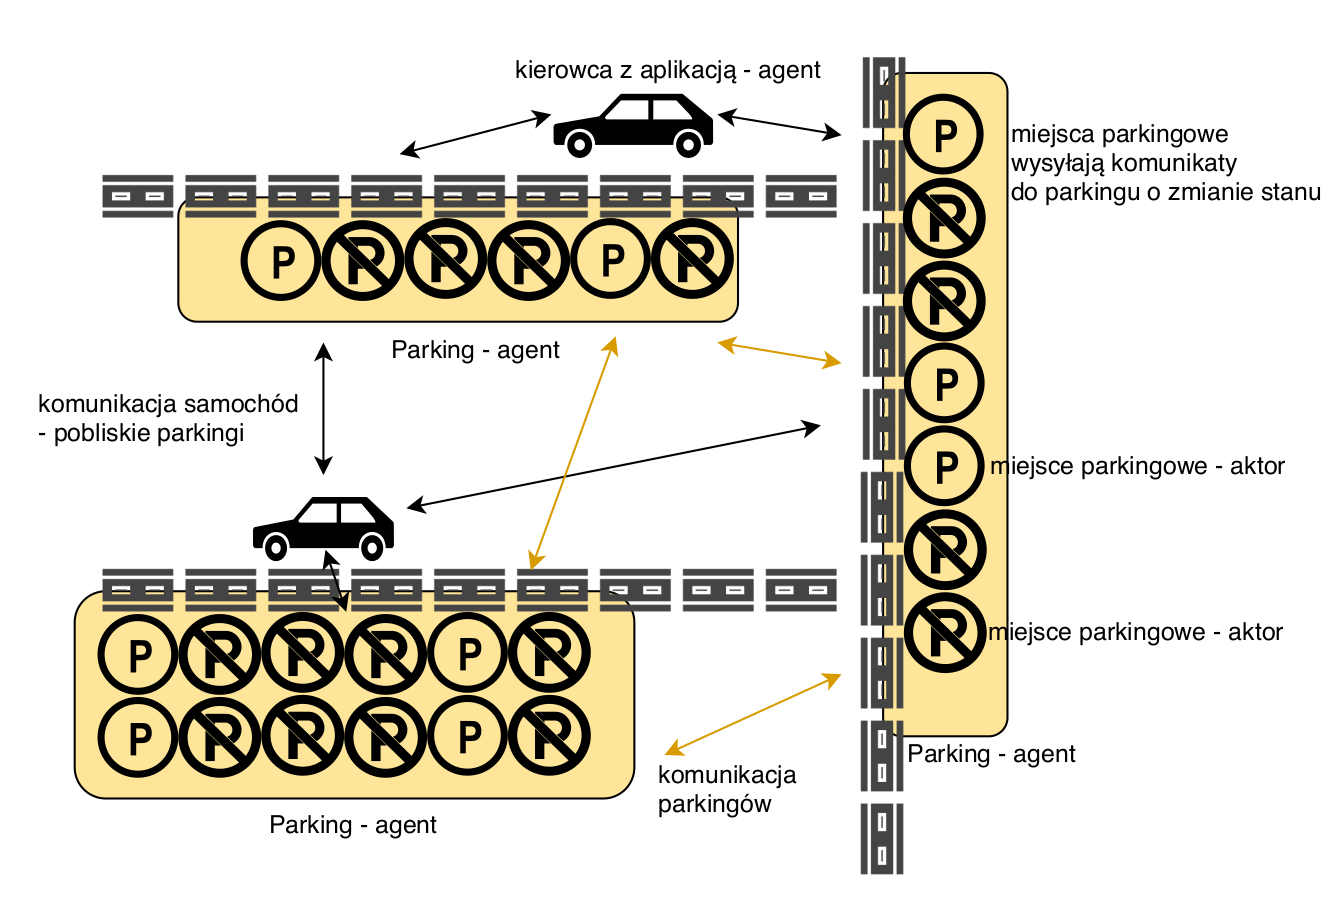
\includegraphics[width=1.1\linewidth]{archi.png}
    \caption{Architektura systemu.}
\end{figure}
